
\section{Shogun}
\subsection{Setup}
\textbf{Preparing the recording space}
\begin{enumerate}
    \item Turn on the electricity for the Vicon cameras
    \item Shut the curtains \textit{completely}
    \item Start up Shogun Live
    \item Turn on the tv screen and duplicate the Shogun window to the screen
\end{enumerate}
\textbf{Preparing the actor}
\begin{enumerate}
    \item Find a suit that fits the actor
    \item Setup the markers on the suit as follows (a Frontwaist10finger marker setup, fig \ref{suit}):
    \begin{figure}[b!]
        \centering
        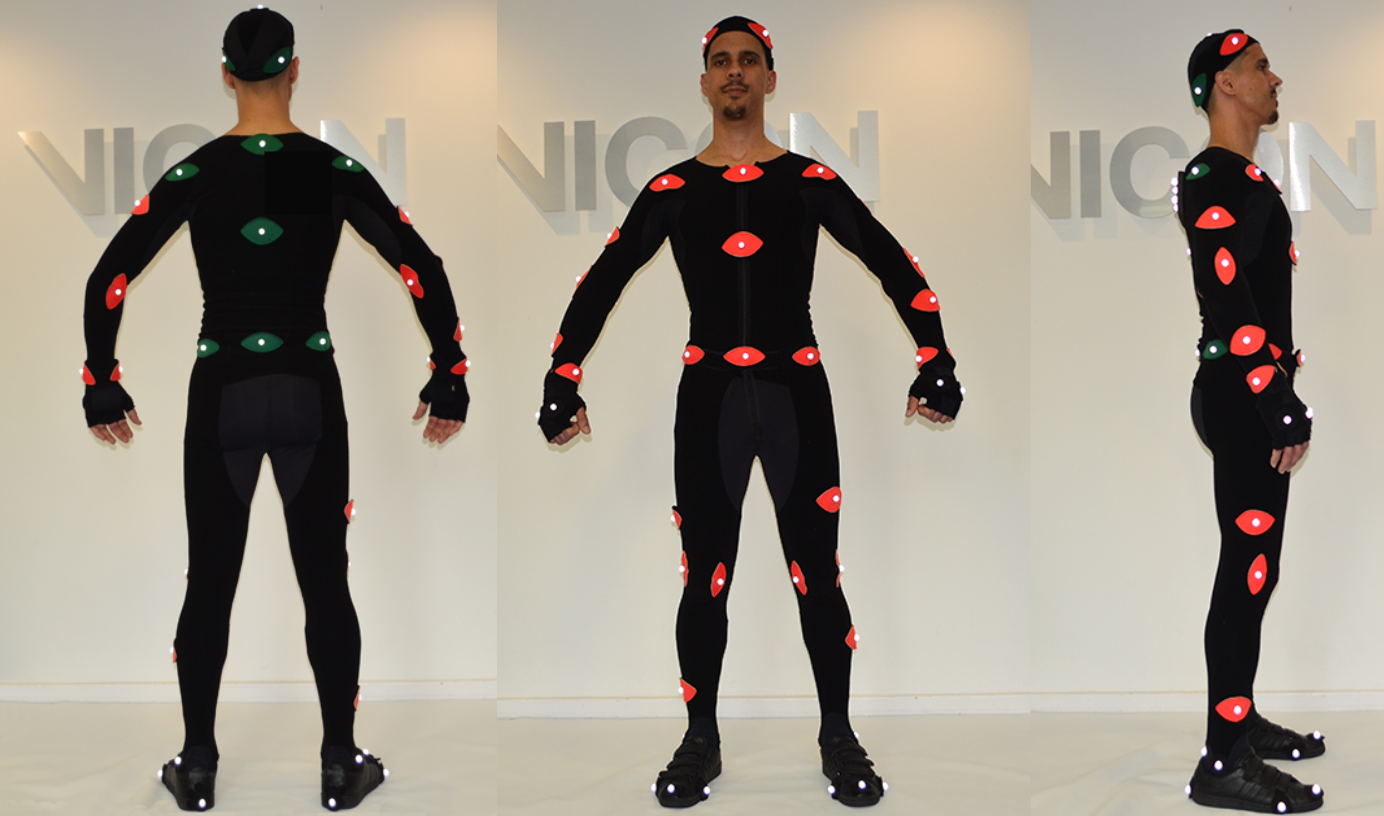
\includegraphics[width=1\linewidth]{imgs/suit/MarkerPlacemtAll.png}
        \caption{The 53 markers on the body}
        \label{suit}
    \end{figure}
    \item Setup the finger markers as follows (make sure to press the bases down on the nails, fig \ref{hands}):
    \begin{figure}[t!]
        \centering
        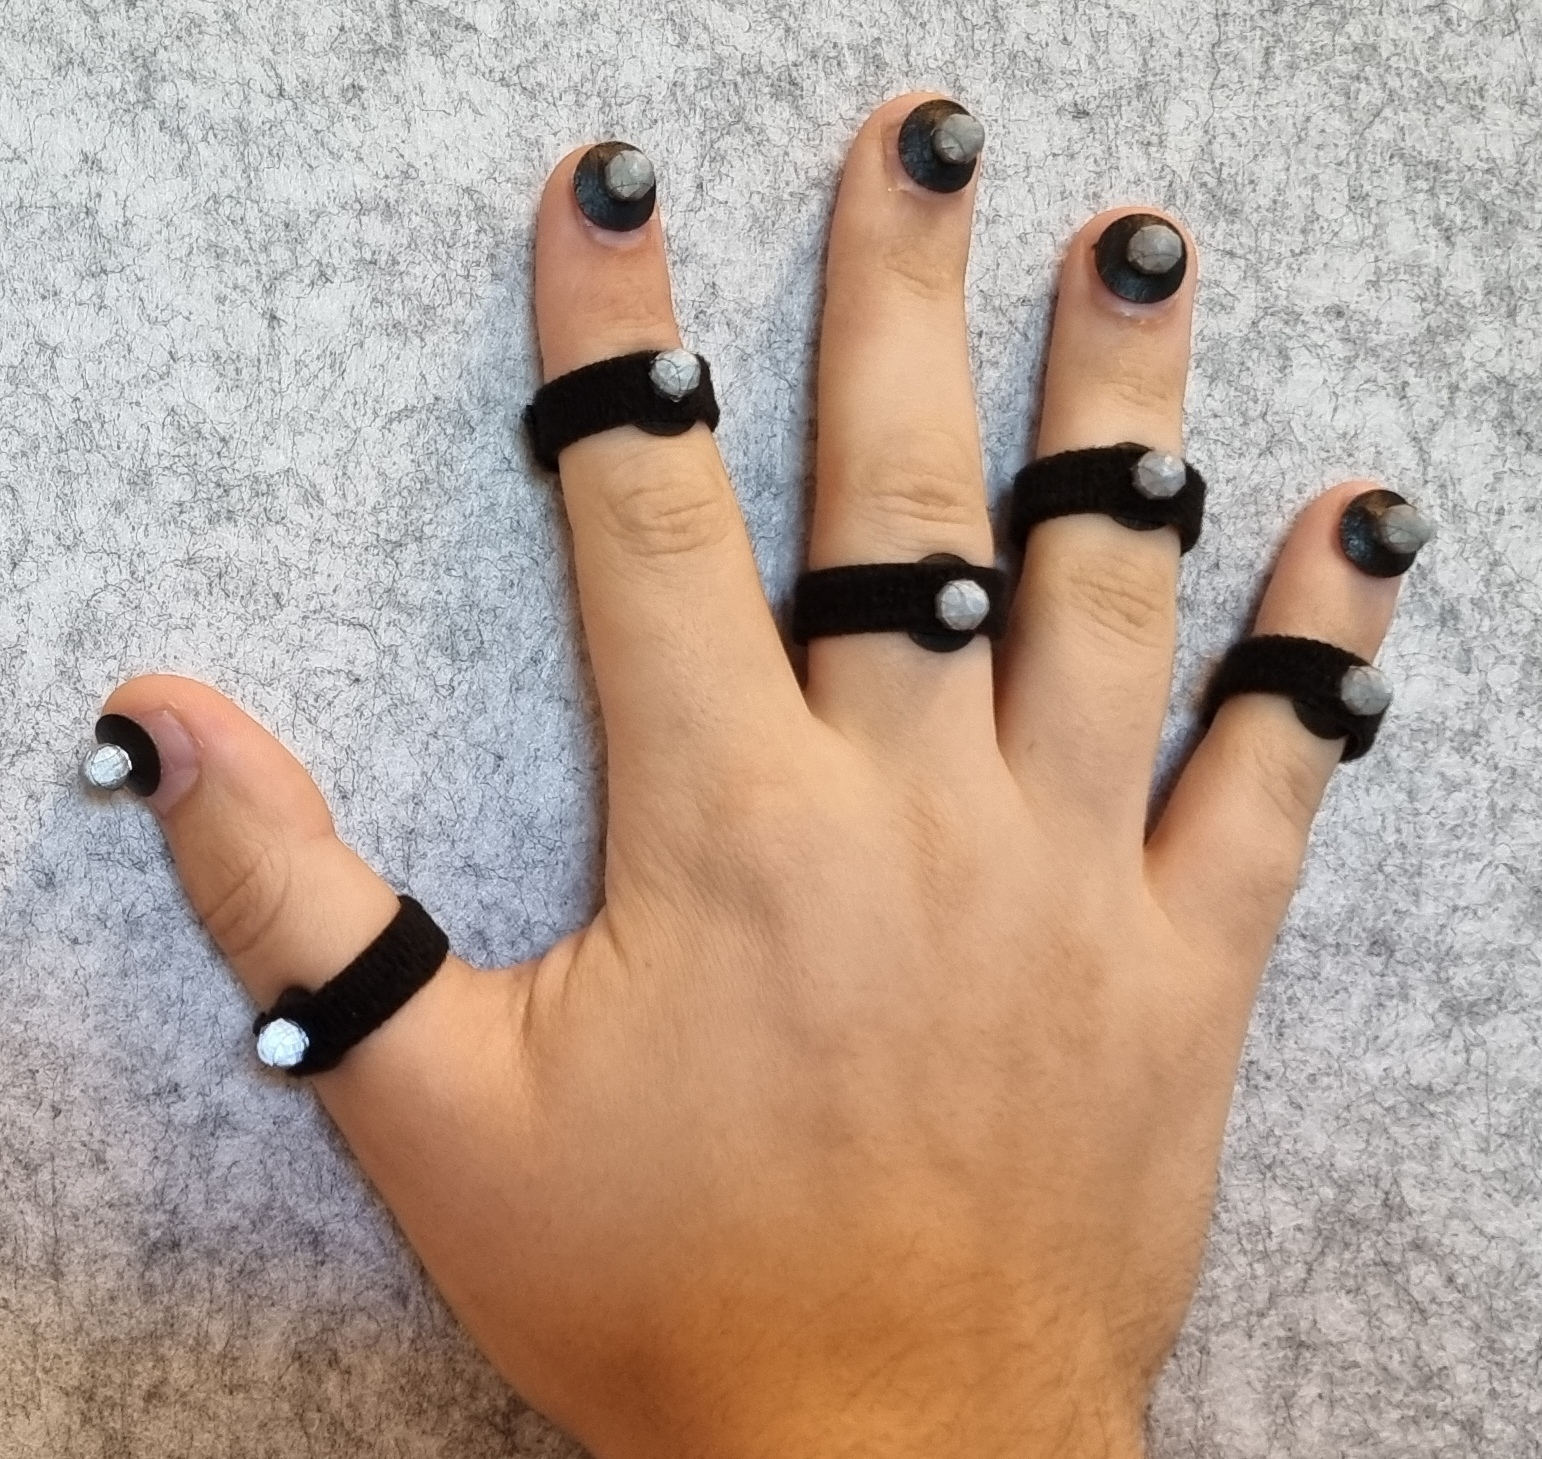
\includegraphics[width=0.5\linewidth]{imgs/suit/fingerSetup.jpg}
        \caption{The 10 finger markers}
        \label{hands}
    \end{figure}
\end{enumerate}
\subsection{Check system health}
\begin{enumerate}
    \item Check for errors for the cameras.\\Hovering over the error symbols will give more info.\\This is how they look:
    
\includegraphics[width=0.03\textwidth]{imgs/icons/icnBumped.png}
    
\includegraphics[width=0.03\textwidth]{imgs/icons/icnCamError.png}
    
\includegraphics[width=0.03\textwidth]{imgs/icons/icnConnectedNotContrib.png}
    
\includegraphics[width=0.03\textwidth]{imgs/icons/icnDisabled.png}
    
\includegraphics[width=0.03\textwidth]{imgs/icons/icnDisconnect.png}
    
\includegraphics[width=0.03\textwidth]{imgs/icons/icnUncal.png}
    \item Check for reflections in the camera view.\\
    Make sure all markers are out of any camera's view and make sure there are no big reflections present. Hide anything reflective if necessary.
\end{enumerate}
\newpage
\subsection{Calibrate}
\textbf{In the Camera calibration tab}
\begin{enumerate}
    \item Mask all
    \item Wave all\\
    The cameras indicate when you are done calibrating them:
    \begin{itemize}
        \item No or purple light: needs to be calibrated
        \item Green: this camera is done calibrating
        \item Blue: all cameras done calibrating
    \end{itemize}
    \item Volume setup
\end{enumerate}

\textbf{In the Tracking tab}
\begin{enumerate}
    \item Turn off all Props and Subjects
    \item Create a new subject by going over the following steps (even when we have an actor that has already been calibrated on a different moment):
    \begin{itemize}
        \item Template: frontwaist10fingers
        \item Name: any name without special characters will do
        \item Create subject
        \item Let the actor do an a-pose (see figure \ref{suit}, but make sure the fingers are relaxed)
        \item Click accept a-pose
        \item Let the actor perform the alphabet, and make them move around until all the joints values are green within Shogun Live
        \item Click Stop Calibrating
    \end{itemize}
    \item \textcolor{red}{What if markers are missing?} Count to make sure there are 73 markers total: 53 on the body a 10 on each hand. Also make sure you placed them at the correct locations, Shogun will tell you what markers are misplaced or missing.
    \item \textcolor{red}{What if there are bones missing in the warning tab?} Make sure the actor is standing in the middle in an a pose. If that is not enough, most likely markers are misplaced.
    \item Go into Properties and select the skin: ViconMaleFingers\_v2
\end{enumerate}

\subsection{Record}
\textbf{In the Capture tab}
\begin{enumerate}
    \item Select the correct recording folder or create the correct folder (make sure to do dd-mm-yyyy)
    \item Capture Name: ROM
    \item Start Capture, ask the Actor to do the alphabet again
    \item Stop the recording
\end{enumerate}

\subsection{Retargeting}
\begin{enumerate}
    \item Open Shogun Post
    \item Open a file, select the file type .mcp, open the ROM just recorded
    \item In the Subject Setup tab, click the Subject Setup button
    \item In the Subject Setup window, go to Retargeting, then in the top left open a previous retarget named: RPM\\
    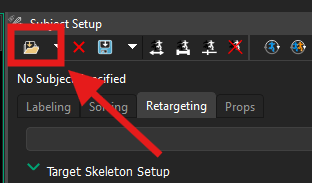
\includegraphics[width=0.25\textwidth]{imgs/openTake.png}
    \item Go into map mode, and then:
    \begin{itemize}
        \item Align Skeletons button
        \item Move and scale the purple skeleton \underline{by its hips (not other bones)} so the wrist positions match
        \item Unscale
        \item Update offsets
        \item Click map mode to go out of map mode
    \end{itemize}
    \item In the top of the Subject Setup window click retarget over playrange
    \item Review the retargeted animation
    \item Save the retarget setup if satisfied, make sure to name it something you remember
    \item Close Shogun Post and go back into Shogun Live
    \item In the tracking tab, select the actor and go into properties (make sure one actor is enabled and the same actor is highlighted)
    \item Select the previously created retarget under Retarget
\end{enumerate}

\subsection{Automatic recording}
\begin{enumerate}
    \item Make sure the PC is connected to the "vislab\_wifi`` wifi network
    \item Run the Vicon\_websocket.bat script
\end{enumerate}